\documentclass[border=0pt]{standalone}
\usepackage[T1]{fontenc}
\usepackage{lmodern}

\usepackage{tikz}

\newdimen\unit
\tikzset{unit/.code={\unit=\dimexpr#1\relax}}
\tikzset{xy/.style={x={#1},y={#1},unit={#1},font={\sffamily\fontsize{.2\unit}{.24\unit}\selectfont},line width=.01\unit}}
\begin{document}%
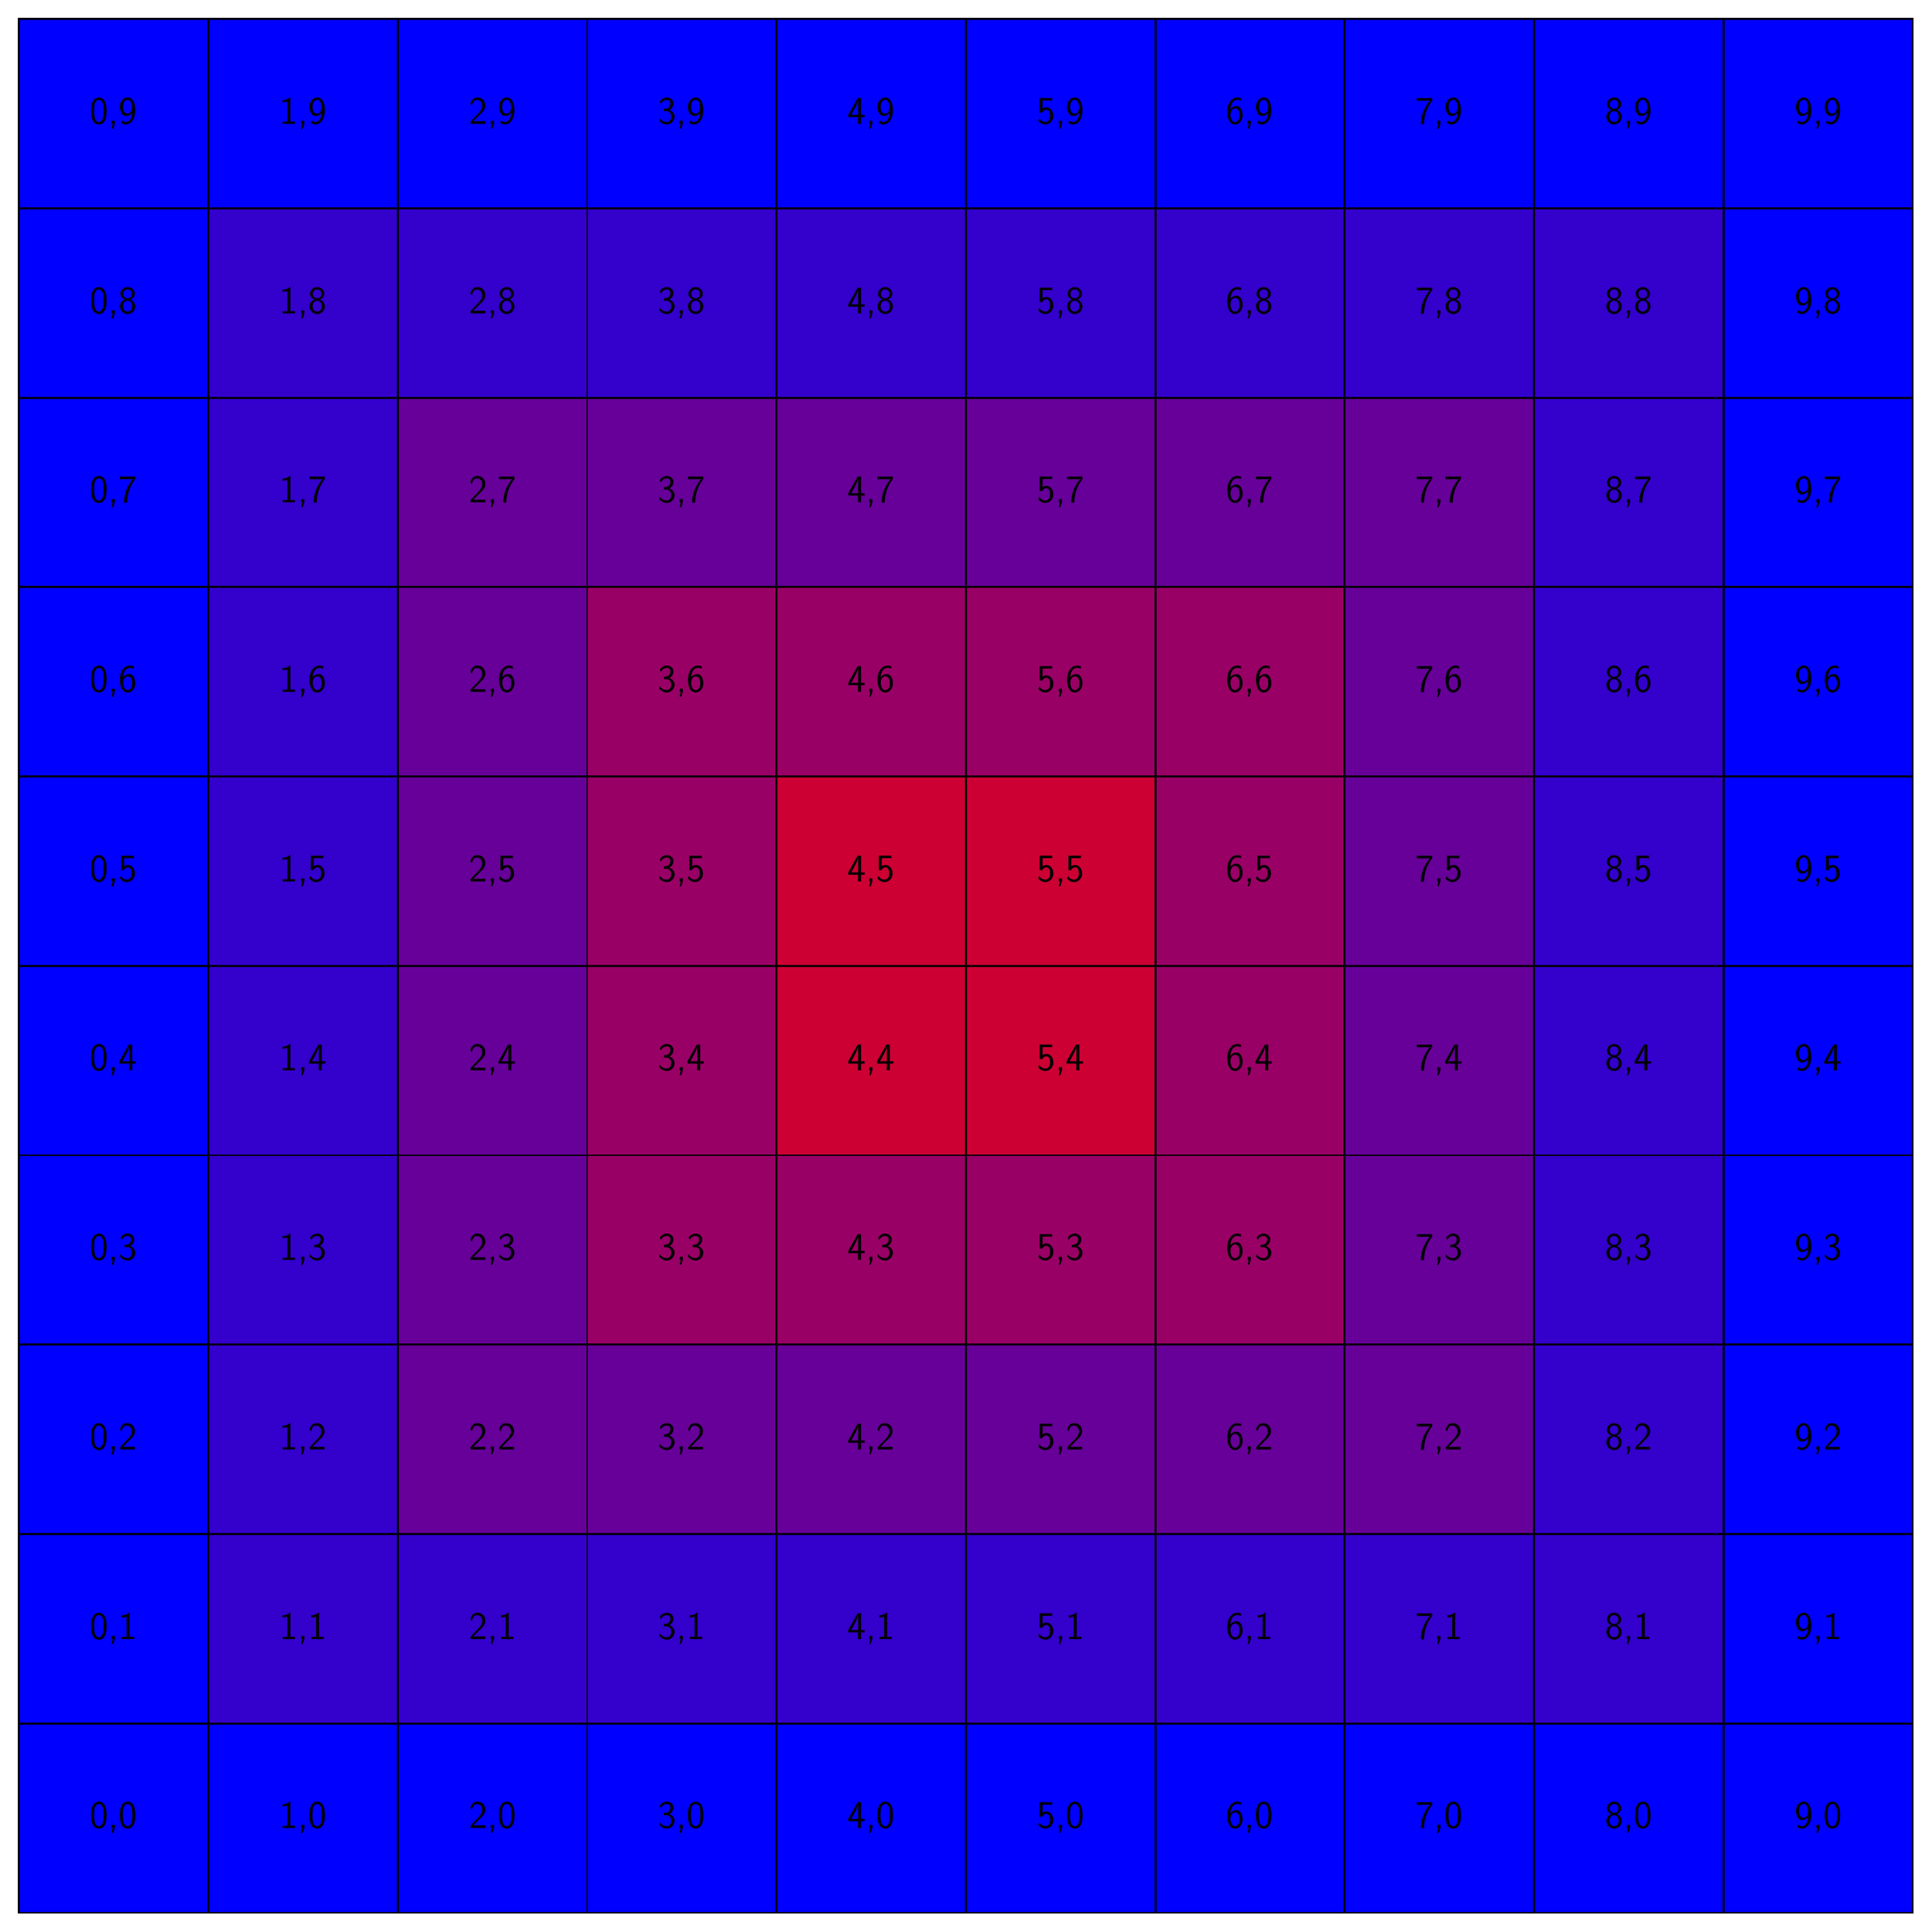
\begin{tikzpicture}[xy=100pt]%
    \path [use as bounding box] (0,0) rectangle (10,10);
    \foreach \x in {5,...,1} {
        \path [fill=blue!\the\numexpr\x*20\relax!red] (5-\x,5-\x) rectangle (5+\x,5+\x);
    }
    \path [draw] (0,0) rectangle (10,10);
    \foreach \x in {0,...,10} {
        \path [draw] (\x,0) rectangle (\x,10);
        \path [draw] (0,\x) rectangle (10,\x);
    }
    \foreach \y in {0,...,9}
    \foreach \x in {0,...,9} {
        \path (\x+.5,\y+.5) node {\x,\y};
    }
\end{tikzpicture}%
\end{document}%
